\section{Пример: данные о твердости зубов}

\footnote{Материал этого раздела является продвинутым, поэтому он может быть пропущен при первом прочтении}
Мы завершаем эту главу рассмотрением более сложного примера, который покажет как возможности, так и ограничения непараметрических $\bca$ и $\abc$ доверительных интервалов.

В таблице 14.3 можно увидеть данные о твердости зубов. Тринадцать человек, попавших в некоторые происшествия потеряли от одного до четырех здоровых зубов. Твердость удалённых зубов была оценена деструктивным исследованием, что в стандартных условиях неосуществимо. <<Твердость>> в последнем столбце таблицы 14.3 --- измеренный для каждого пациента показатель средней твердости зубов (в логарифмической шкале).

\noindent
\begin{center}
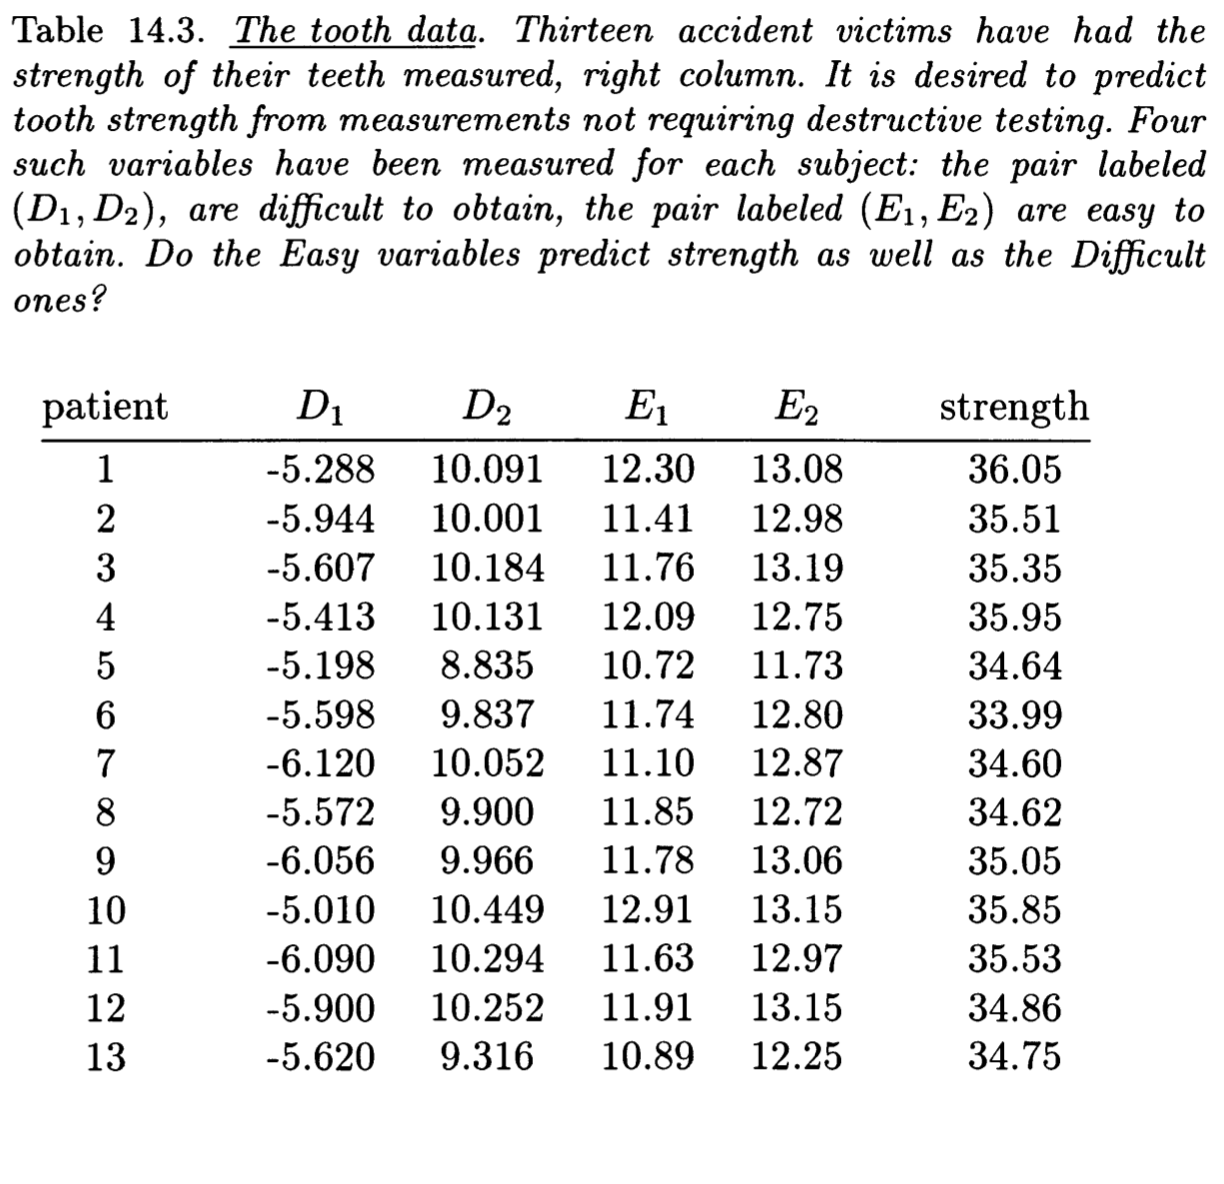
\includegraphics[width=0.9\linewidth]{14/t143.png}
\end{center}
\setcounter{table}{3}

Исследователи хотели предсказать твердость зубов используя переменные, которые не требуют разрушения зубов и могут быть измерены на рутинных осмотрах. В таблице 14.3 показаны данные о четырех таких переменных --- $D_1$, $D_2$, $E_1$, $E_2$. Пару $(D_1, D_2)$ трудно и дорого получить, а пару $(E_1, E_2)$ --- легко и дешево. Исследователи задались следующим вопросом: насколько хорошо <<простые>> переменные $(E_1, E_2)$ предсказывают твердость зубов в сравнении с <<труднодоступными>> $(D_1, D_2)$.

Данный вопрос можно формализовать используя линейные модели, как в главах 7 и 9. Каждая строка $x_i$ матрицы данных из таблицы 14.3 состоит из пяти чисел: двух $D$, двух $E$, а также значения твердости, то есть
\begin{equation}
  x_i = (d_{i1}, d_{i2}, e_{i1}, e_{i2}, y_i) \qquad (i = \ies{13}).
\end{equation}
Пусть $\mbf D$ --- матрица, использующая только переменные $D$ для предсказания $y_i$ с помощью линейной регрессии (включая сдвиг), то есть $\mbf D$ --- матрица $13 \times 3$ с $i$-й строкой вида
\begin{equation}
  (1, d_{i1}, d_{i2}).
\end{equation}

Оценка $y_i$ по методу наименьших квадратов на основе переменных $D$ имеет вид
\begin{equation}
  \what y_i(D) = \what \beta_0(D) + \what \beta_1(D) d_{i1} + \what \beta_2(D) d_{i2},
\end{equation}
где вектор $\what \beta (D) = (\what \beta_0(D),\what \beta_1(D) , \what \beta_2(D))$ есть решение задачи наименьших квадратов
(9.28), то есть
\begin{equation}
  \what \beta (D) = (\mbf D^\mathrm{T} \mbf D)^{-1} \mbf D^\mathrm{T}\mbf y,
\end{equation}
где $y = (y_1,y_2,\ldots,y_{13})$. $\tx{RSE}(D)$ (residual squared error) есть сумма квадратов ошибок между предсказаниями $\what y_i (D)$ и наблюдениями $y_i$ для $n = 13$ пациентов
\begin{equation}
  \tx{RSE}(D) = \summ{i=1}{N} (y_i - \what y_i (D))^2.
\end{equation}
Меньшие значения $\tx{RSE}$ являются индикатором хорошего качества предсказания; наилучшее возможное значение $\tx{RSE} = 0$ достигается на идеальном предсказании для каждого из пациентов.

Аналогичнным образом мы можем предсказывать $y_i$, используя только переменные $E$ и в результате вычислить
\begin{equation}
  \tx{RSE}(E) = \summ{i = 1}{n}(y_i - \what y_i(E))^2.
\end{equation}
Вопрос исследователя о том, насколько переменные двух разных типов, $D$ и $E$, сравнимы по качеству предсказания, может быть переформулирован как вопрос о сравнении \tx{RSE}(D) и \tx{RSE}(E). Практичная в атком случае статистика имеет вид
\begin{equation}
  \what \theta = \frac{1}{n} [\tx{RSE}(E) - \tx{RSE}(D)].
\end{equation}
Положительное значение $\what \theta$ означало бы, что переменные $E$ хуже чем переменные $D$ в предсказании твердости. (Если бы число измерений $E$ и $D$ не совпадают, то статистика $\what \theta$ должна быть преобразована). %см. задачу 14.12 
Были получены значения $\tx{RSE}(D) = 2.761$ и $\tx{RSE}(E) = 3.130$, что приводит к
\begin{equation}
  \what \theta = 0.0285.
\end{equation}
Это свидетельствует о том, что переменные $D$ являются более предпочтительными для предсказания, так как $\what \theta$ больше нуля, однако мы не можем быть уверены в этом, пока не оценим статистическую изменчивость $\what \theta$. Для этого мы используем методы $\bca$ и $\abc$. Рисунок 14.4 указывает на то, что ситуация может оказаться <<пограничной>>, так как предсказанные значения $\what y_i(D)$ и $\what y_i(E)$ близки для каждого из наблюдений. Также следует заметить, что разница между $\tx{RSE}(D)$ и $\tx{RSE}(E)$ составляет около $10\%$ от самих значений $\tx{RSE}$. Поэтому даже если эта разница статистически значима, она может быть не сильно важной в практическом плане. Построение доверительного интервала позволит ответить как на вопрос значимости, так и на вопрос важности этой разницы.
 

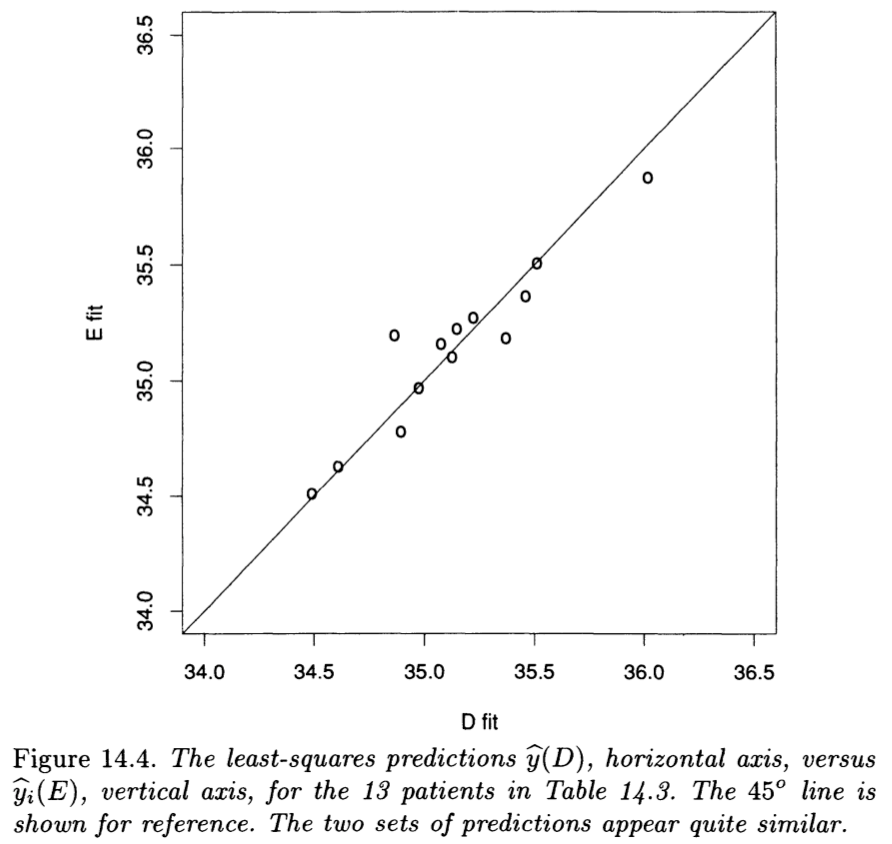
\includegraphics[width=0.85\linewidth]{14/f144.png}
\newline

В левой части рисунка 14.5 --- гистограмма 2000 репликаций непараметрического бутстрепа статистики RSE разности $\what \theta$, (14.31). Пусть $\mbf x = (\xes{13})$ представляет из себя матрицу данных из таблицы 14.3, где $x_i$ есть $i$-ый столбец матрицы, (14.25). Непараметрическая бутстреп выборка $\mbf x^* = (\xest{13})$ есть матрица, состоящая из строк, взятых с возвращением из совокупности $\{\xes{13}\}$. Это эквивалентно следующей записи:
\begin{equation}
  \what F \rightarrow\mbf x^* = (\xest{13}),
\end{equation}
где $\what F$ есть эмпирическая функция распределения, которая задает вероятность $1/13$ выбора каждой из строк $x_i$.

Следуя определениям из (14.25)--(14.30) бутстреп матрица $\mbf x^*$ приводит к $\mbf y^*$, $\mbf D^*$, $\what \beta(D)^*$, $\what y_i (D)^*$, а затем

\begin{equation}
  \rse(D)^* = \summ{i = 1}{13} (y_i^* - \what y_i(D)^*)^2,
\end{equation}
и аналогично $\rse(E)^* = \summ{i = 1}{13} (y_i^* - \what y_i(E)^*)^2$. Бутстреп репликация $\what \theta$ будет иметь вид
\begin{equation}
  \what \theta^* = \frac{1}{13}[\rse(E)^* - \rse(D)^*].
\end{equation}
Как и всегда, $\what \theta^*$ вычисляется с помощью того же алгоритма, что и исходная оценка $\what \theta$. Меняется лишь матрица данных $\mbf x$ на $\mbf x^*$ и вектор $\mbf y$ на $\mbf y^*$. 

Бутстреп гистограмма содержит информацию, которая нам необходима для ответа на вопросы  о значимости и важности $\what \theta$. Даже без построения доверительных интервалов можно получить некоторые ответы. Бутстреп оценка стандартной ошибки (6.6) равна
\begin{equation}
  \what{\tx{se}}_{2000} = 0.0311.
\end{equation}
Это означает, что $\what \theta = 0.0285$ менее чем на одну стандартную ошибку отстоит от нуля, откуда можно сделать вывод о том, что нам не следует ожидать серьезных оснований отвергнуть гипотезу о том, что истинное значение $\theta$ равно 0. С другой стороны, оценка смещена вниз ($62\%$ значений $\what \theta^*$ оказываются меньшими, чем $\what \theta^*$). Это указывает на то, что уровень значимости окажется больше $0.18 = 1 - \Phi(0.0285/0.0311)$, в условиях нормальной аппроксимации $\what \theta \sim N(\theta,0.0311^2)$.

Бутстреп гистограмма указывает на то, что $\theta$ оказывается не более $0.10$. Насколько существенна эта разница? Для этого нужно понять что именно измеряет параметр $\theta$.    Если $F$ есть истинное пятимерное распределение вектора $(d_1,d_2,e_1,e_2,y)$, то
\begin{align}
	\theta_D &= \min_{\beta_D} \tx{E}_F [y - (\beta_{D_0} + \beta_{D_1}d_1 + \beta_{D_0}d_2)]^2, \notag\\
	\theta_E &= \min_{\beta_E} \tx{E}_F [y - (\beta_{E_0} + \beta_{E_1}e_1 + \beta_{E_0}e_2)]^2
\end{align}
--- есть истинное значение ошибок предсказания при использовании переменных $D$ и $E$, соответственно. Параметр $\theta$, соответствующий $\what \theta$ есть
\begin{equation}
  \theta = \theta_E - \theta_D.
\end{equation}
Оценка $\theta_D$ по методу подстановки --- $\what \theta_D = \rse(D)/13 = 0.212$. Наша гипотеза о том, что $\theta \leqslant 0.10$ приводит к 
\begin{equation}
  \frac{\theta_E - \theta_D}{\theta_D} \dot = \frac{\theta_E - \theta_D}{\what \theta_D} < \frac{0.10}{0.212} = 0.47.
\end{equation}
Можно сделать вывод о том, что переменные E вероятно не лучше, чем переменные D для предсказания твердости, и вероятно не более чем на $50\%$ хуже.

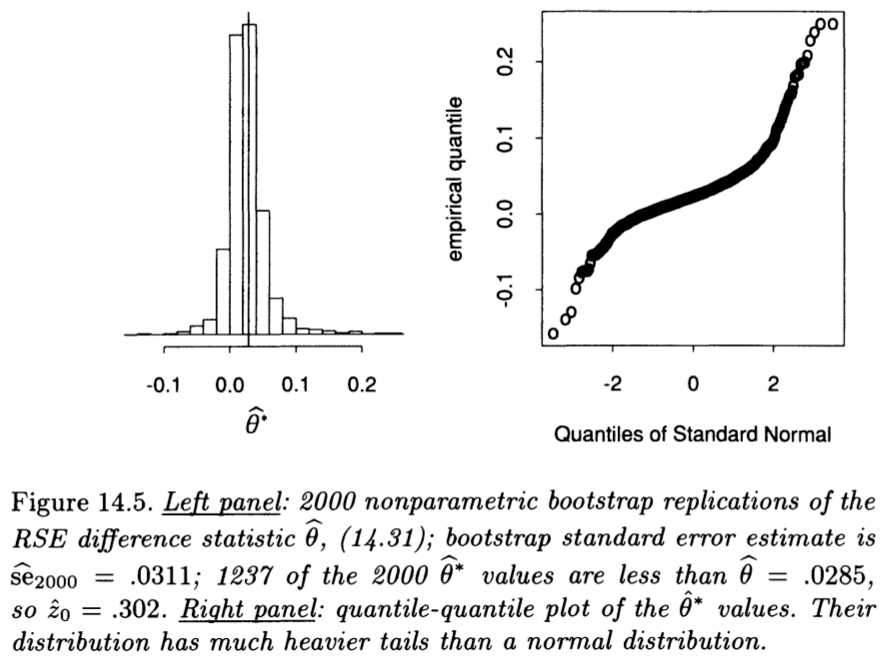
\includegraphics[width=0.85\linewidth]{14/f145.png}
\newline

В первом столбце таблицы 14.4 указаны доверительные интервалы для $\theta$ по методу $\bca$ на основе 2000 репликаций непараметрического бутстрепа.

Доверительные границы $\what \theta[\alpha]$ даны для восьми значений уровня значимости. Доверительные интервалы получаются взятием пар вида $(\what \theta[\alpha], \what \theta[1-\alpha])$ (например, $(\what \theta[0.05], \what \theta[0.95])$ --- $90\%$ интервал). Формулы (14.14) и (14.15) приводят к малому значению ускорения и большой поправке на смещение --- $\hat a = 0.040$ и $\hat z_0 = 0.47$.

Заметим, что непараметрическая граница для 0.05 положительна, $\what \theta[0.05] = 0.004$. Как говорилось ранее, это связано с большим значением поправки на смещение. Если бы $\bca$ метод был точным, мы могли бы утверждать, что нулевая гипотеза $\theta = 0$ отвергается при односторонеей критической области и уровне значимости $0.05$. Метод не точный, поэтому следует быть осторожнее с выводами. Непараметрические $\bca$ интервалы часто оказываются немного короткими, в особенности в случаях малой выборки (как в этом примере). Если бы проверка гипотезы имела критическое значение, то возможно добиться улучшения уровня значимости посредством калибровке, как в разделе 25.6.

\noindent
\begin{center}
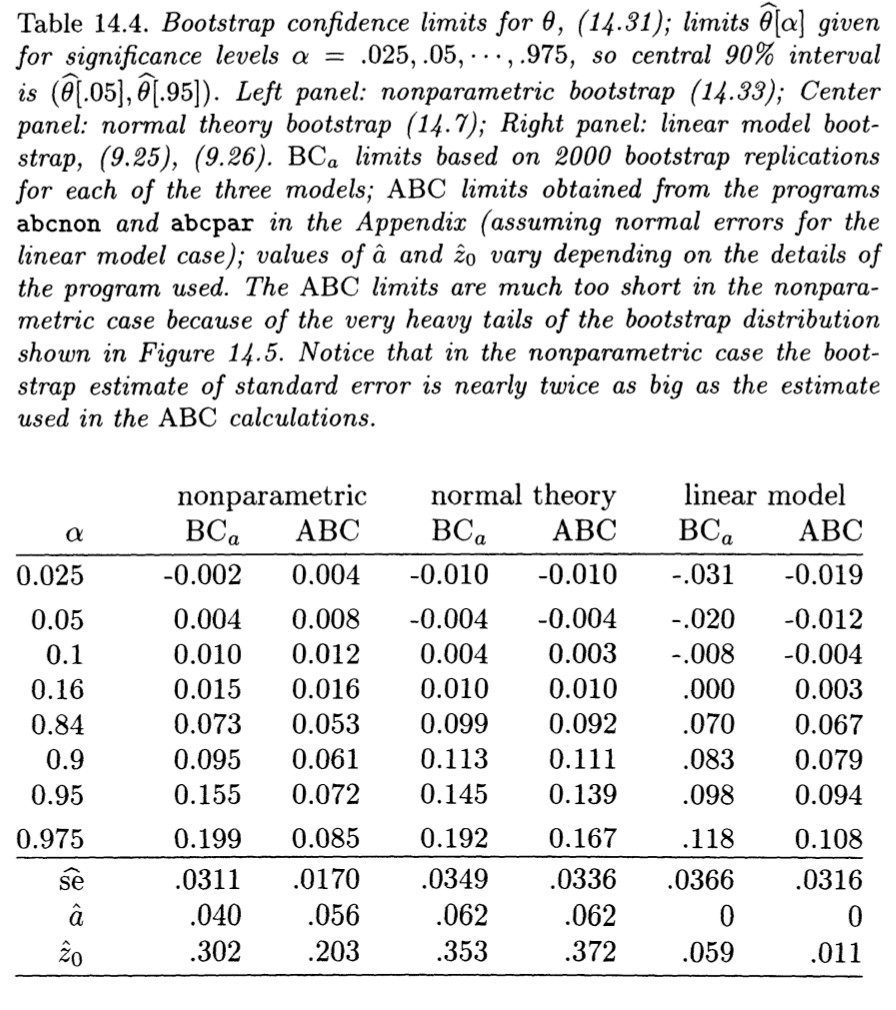
\includegraphics[width=0.9\linewidth]{14/t144.png}
\end{center}
\setcounter{table}{3}

Для проверки непараметрических интервалов было построено еще 2000 бутстреп выборок, в данном случае основанных на нормальной модели; предполагается, что строки $x_i$ матрицы данных были получены моделированием из пятимерного нормального распределения $F_\tx{norm}$. Далее было найдено наилучшее аппроксимирующее данные распределение $\what F_\tx{norm}$, а затем сгенерированы выборки $\mbf x^*$ из $\what F_\tx{norm}$ как в (14.7). Гистограмма на основе 2000 бутстреп репликаций параметрического бутстрепа показана на левой стороне рисунка 14.6; она похожа на гистограмму из рисунка 14.5 (за исключением того, что в данном случае хвосты менее тяжелые).

$\bca$ интервалы вычислены так же, как и ранее, используя формулы (14.9) и (14.10). Формула поправки на смещение (14.14) также не изменилась. Параметр ускорения $\hat a$ вычислен с помощью параметрической версии формулы (14.15), взятой из алгоритма \texttt{abcpar} построения параметрических $\abc$ интервалов. В данном случае параметрические $\bca$ границы, указанные в центральной части таблицы 14.4, не сильно отличаются от своего непараметрического аналога. В то же время разница оказывается достаточно большой, такой, что гипотеза $\theta = 0$ уже не отвергается на уровне $0.05$ (при выборе одностороннего доверительного интервала).

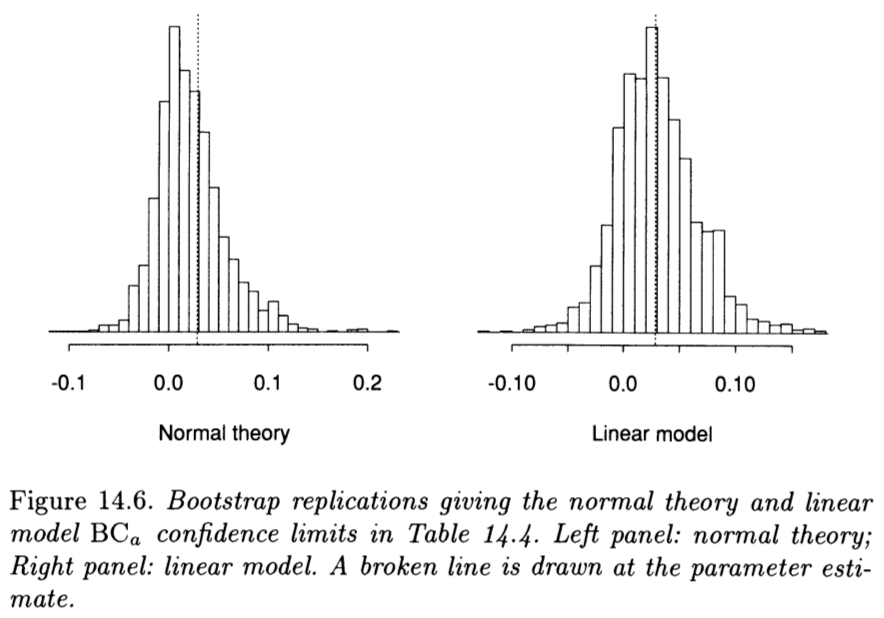
\includegraphics[width=0.85\linewidth]{14/f146.png}
\newline

Непохоже, что исходные данные распределены нормально. Однако причиной использования бутстрепа с предположением нормальности заключается в малой размерности данных, $n=13$. Для слишком малых выборок бутстреп даже с неподходящей параметрической моделью может оказаться более успешным, уменьшив дисперсию результатов в ущерб допустимого смещения. В данном же примере результаты по двум методам весьма похожи.

В главе 9 рассматриваются модели линейной регрессии. Можем использовать модель линейной регрессии для того, чтобы предложить другой вариант бутстреп анализа разностной статистики $\hat \theta$. Используя обозначения из (14.25), пусть $c_i$ представляет из себя вектор
\begin{equation}
 \mbf c_i = (1,d_{1i},d_{2i}, e_{1i}, e_{2i});
\end{equation}
рассмотрим линейную модель (9.4), (9.5)
\begin{equation}
  y_i = \mbf c_i\mbf \beta + \varepsilon_i \qquad (\ies{13}).
\end{equation}
Бутстреп выборки $\mbf y^* = (y_1^*,y_2^*,\ldots,y_{13}^*)$ получены из остатков повторных выборок (как в (9.25) и (9.26)). Бутстреп репликации $\what \theta^*$ остаются такими же, как в (14.35). Следует заметить, что вычисление $\what y_i(D)^*$ и $\what y_i(E)^*$ несколько отличается.

На правой стороне рисунка 14.6 показано бутстреп распределение на основе 2000 репликаций $\what \theta^*$. Хвосты  у этой гистограммы легче, чем хвосты на рисунке 14.5. Это отражено и в таблице 14.4 --- соответствующие интервалы стали более узкими. Несмотря на это, гипотеза $\theta = 0$ 	отвергается реже, чем раньше: при уровне $\alpha = 0.16$. Это происходит из-за того, что $\what \theta$ уже не выглядит смещенной вниз, $\what z_0$ равен $0.059$, а не $0.302$, как в непараметрическом случае.

Доверительные интервалы и проверка гипотез являются <<деликатными>> инструментами статистической теории выводов. В этой связи они сильнее зависят от выбора модели, чем обычные стандартные ошибки. В особенности эти соображения верны для случаев, когда размер выборки мал. Исследование зависимостей между пятью переменными на основе 13 наблюдений очевидно является задачей с малым размером выборки. Даже если бы $\bca$ интервалы были точными (а это не так), то изменение модели приводило бы к другим доверительным интервалам, что видно из таблицы 14.4.

В таблице 14.4 показаны $\abc$ интервалы для трёх различных вариантов выбора модели. Результаты были получены с использованием реализаций программ \texttt{abcnon} и \texttt{abcpar} из приложения. Непараметрические $\abc$ интервалы оказываются слишком короткими в данном случае. Это происходит из-за необычно тяжелых хвостов у распределения непараметрического бустстрепа. Если говорить на языке статистики, то метод $\abc$ может исправить асимметрию распределения, но не его эксцесс (это все, что требуется для достижения точности второго порядка). Асимптиотическая точность метода $\abc$ не гарантирует его успешность на малых выборках.

Стандартные ошибки $\what \theta$ даны для каждого из шести столбцов в таблице 14.4. Приведенные для $\bca$ --- это классические бутстреп стандартные ошибки. Стандартные ошибки для $\abc$ получены с помощью дельта метода из главы 21 (похожего на метод вычисления стандартной ошибки по методу складного ножа, (11.5)). Стандартная ошибка $\bca$ более чем в два раза превышает ошибку по методу $\abc$ в непараметрическом случае, что свидетельствует о том, что интервалы $\abc$ будут слишком короткими. (Большая $\bca$ стандартная ошибка стала заметна уже после первых 100 бутстреп репликаций.) Обычно аппроксимация по методу $\abc$ работает удовлетворительно как в таблице 14.2. Однако в любом случае может оказаться полезной проверка стандартных ошибок используя небольшое число бутстреп репликаций (например, 100).

 




